\documentclass{standalone}
\usepackage{tikz}
\usetikzlibrary{patterns, positioning}


\begin{document}
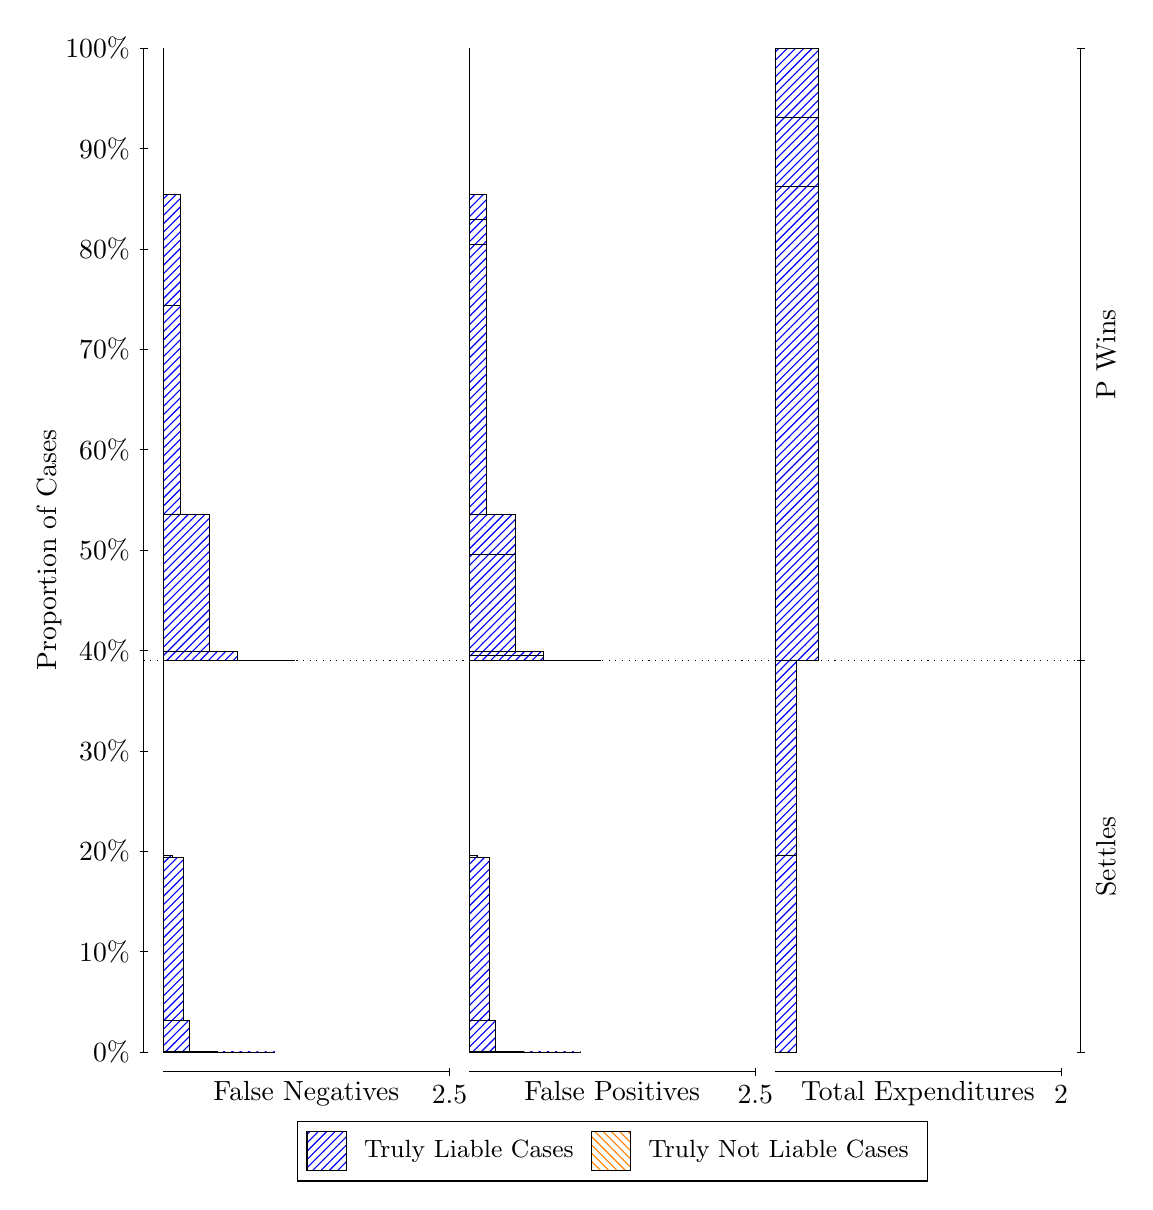
\begin{tikzpicture}
\draw[black, very thin] (1.5,1.75) -- (1.5,14.5);
\node[rotate=90, text=black, anchor=center] at (0.3, 8.125) {Proportion of Cases};
\draw[black, very thin] (1.45,1.75) -- (1.55,1.75);
\node[text=black, anchor=east] at (1.45, 1.75) {0\%};
\draw[black, very thin] (1.45,3.025) -- (1.55,3.025);
\node[text=black, anchor=east] at (1.45, 3.025) {10\%};
\draw[black, very thin] (1.45,4.3) -- (1.55,4.3);
\node[text=black, anchor=east] at (1.45, 4.3) {20\%};
\draw[black, very thin] (1.45,5.575) -- (1.55,5.575);
\node[text=black, anchor=east] at (1.45, 5.575) {30\%};
\draw[black, very thin] (1.45,6.85) -- (1.55,6.85);
\node[text=black, anchor=east] at (1.45, 6.85) {40\%};
\draw[black, very thin] (1.45,8.125) -- (1.55,8.125);
\node[text=black, anchor=east] at (1.45, 8.125) {50\%};
\draw[black, very thin] (1.45,9.4) -- (1.55,9.4);
\node[text=black, anchor=east] at (1.45, 9.4) {60\%};
\draw[black, very thin] (1.45,10.675) -- (1.55,10.675);
\node[text=black, anchor=east] at (1.45, 10.675) {70\%};
\draw[black, very thin] (1.45,11.95) -- (1.55,11.95);
\node[text=black, anchor=east] at (1.45, 11.95) {80\%};
\draw[black, very thin] (1.45,13.225) -- (1.55,13.225);
\node[text=black, anchor=east] at (1.45, 13.225) {90\%};
\draw[black, very thin] (1.45,14.5) -- (1.55,14.5);
\node[text=black, anchor=east] at (1.45, 14.5) {100\%};

\draw[black, very thin] (13.4,1.75) -- (13.4,14.5);
\draw[black, very thin] (13.35,1.75) -- (13.45,1.75);
\node[anchor=west] at (13.35, 1.75) {};
\draw[black, very thin] (13.35,6.7188) -- (13.45,6.7188);
\node[anchor=west] at (13.35, 6.7188) {};
\draw[black, very thin] (13.35,14.5) -- (13.45,14.5);
\node[anchor=west] at (13.35, 14.5) {};

\draw[black, very thin, pattern color=blue, pattern=north east lines] (1.75,1.75) rectangle (3.167,1.75);
\draw[black, very thin, pattern color=blue, pattern=north east lines] (1.75,1.75) rectangle (2.8763,1.75);
\draw[black, very thin, pattern color=blue, pattern=north east lines] (1.75,1.75) rectangle (2.8037,1.75);
\draw[black, very thin, pattern color=blue, pattern=north east lines] (1.75,1.75) rectangle (2.5857,1.75);
\draw[black, very thin, pattern color=blue, pattern=north east lines] (1.75,1.75) rectangle (2.513,1.75);
\draw[black, very thin, pattern color=blue, pattern=north east lines] (1.75,1.75) rectangle (2.4403,1.7532);
\draw[black, very thin, pattern color=blue, pattern=north east lines] (1.75,1.7532) rectangle (2.295,1.7532);
\draw[black, very thin, pattern color=blue, pattern=north east lines] (1.75,1.7532) rectangle (2.2223,1.7539);
\draw[black, very thin, pattern color=blue, pattern=north east lines] (1.75,1.7539) rectangle (2.1497,1.7541);
\draw[black, very thin, pattern color=blue, pattern=north east lines] (1.75,1.7541) rectangle (2.077,2.1555);
\draw[black, very thin, pattern color=blue, pattern=north east lines] (1.75,2.1555) rectangle (2.0043,4.2246);
\draw[black, very thin, pattern color=blue, pattern=north east lines] (1.75,4.2246) rectangle (1.9317,4.2249);
\draw[black, very thin, pattern color=blue, pattern=north east lines] (1.75,4.2249) rectangle (1.859,4.2439);
\draw[black, very thin, pattern color=blue, pattern=north east lines] (1.75,4.2439) rectangle (1.7863,4.2442);
\draw[black, very thin, pattern color=orange, pattern=north west lines] (1.75,4.2442) rectangle (1.75,4.2442);
\draw[black, very thin, pattern color=blue, pattern=north east lines] (1.75,4.2442) rectangle (1.75,6.7188);
\draw[black, very thin, pattern color=blue, pattern=north east lines] (1.75,6.7188) rectangle (3.4213,6.7188);
\draw[black, very thin, pattern color=blue, pattern=north east lines] (1.75,6.7188) rectangle (3.058,6.72);
\draw[black, very thin, pattern color=blue, pattern=north east lines] (1.75,6.72) rectangle (2.6947,6.8398);
\draw[black, very thin, pattern color=blue, pattern=north east lines] (1.75,6.8398) rectangle (2.3313,8.5778);
\draw[black, very thin, pattern color=blue, pattern=north east lines] (1.75,8.5778) rectangle (1.968,11.235);
\draw[black, very thin, pattern color=blue, pattern=north east lines] (1.75,11.235) rectangle (1.968,12.641);
\draw[black, very thin, pattern color=orange, pattern=north west lines] (1.75,12.641) rectangle (1.75,12.641);
\draw[black, very thin, pattern color=blue, pattern=north east lines] (1.75,12.641) rectangle (1.75,14.5);
\draw[black, very thin, pattern color=orange, pattern=north west lines] (5.6333,1.75) rectangle (7.0503,1.75);
\draw[black, very thin, pattern color=blue, pattern=north east lines] (5.6333,1.75) rectangle (7.0503,1.75);
\draw[black, very thin, pattern color=orange, pattern=north west lines] (5.6333,1.75) rectangle (6.7597,1.75);
\draw[black, very thin, pattern color=blue, pattern=north east lines] (5.6333,1.75) rectangle (6.7597,1.75);
\draw[black, very thin, pattern color=blue, pattern=north east lines] (5.6333,1.75) rectangle (6.687,1.75);
\draw[black, very thin, pattern color=orange, pattern=north west lines] (5.6333,1.75) rectangle (6.469,1.75);
\draw[black, very thin, pattern color=blue, pattern=north east lines] (5.6333,1.75) rectangle (6.469,1.75);
\draw[black, very thin, pattern color=blue, pattern=north east lines] (5.6333,1.75) rectangle (6.3963,1.75);
\draw[black, very thin, pattern color=blue, pattern=north east lines] (5.6333,1.75) rectangle (6.3237,1.7531);
\draw[black, very thin, pattern color=orange, pattern=north west lines] (5.6333,1.7531) rectangle (6.1783,1.7531);
\draw[black, very thin, pattern color=blue, pattern=north east lines] (5.6333,1.7531) rectangle (6.1783,1.7531);
\draw[black, very thin, pattern color=blue, pattern=north east lines] (5.6333,1.7531) rectangle (6.1057,1.7538);
\draw[black, very thin, pattern color=blue, pattern=north east lines] (5.6333,1.7538) rectangle (6.033,1.7541);
\draw[black, very thin, pattern color=blue, pattern=north east lines] (5.6333,1.7541) rectangle (5.9603,2.1555);
\draw[black, very thin, pattern color=orange, pattern=north west lines] (5.6333,2.1555) rectangle (5.8877,2.1555);
\draw[black, very thin, pattern color=blue, pattern=north east lines] (5.6333,2.1555) rectangle (5.8877,4.2246);
\draw[black, very thin, pattern color=blue, pattern=north east lines] (5.6333,4.2246) rectangle (5.815,4.2249);
\draw[black, very thin, pattern color=blue, pattern=north east lines] (5.6333,4.2249) rectangle (5.7423,4.2439);
\draw[black, very thin, pattern color=blue, pattern=north east lines] (5.6333,4.2439) rectangle (5.6697,4.2442);
\draw[black, very thin, pattern color=blue, pattern=north east lines] (5.6333,4.2442) rectangle (5.6333,6.7188);
\draw[black, very thin, pattern color=orange, pattern=north west lines] (5.6333,6.7188) rectangle (7.3047,6.7188);
\draw[black, very thin, pattern color=blue, pattern=north east lines] (5.6333,6.7188) rectangle (7.3047,6.7188);
\draw[black, very thin, pattern color=orange, pattern=north west lines] (5.6333,6.7188) rectangle (6.9413,6.7188);
\draw[black, very thin, pattern color=blue, pattern=north east lines] (5.6333,6.7188) rectangle (6.9413,6.7191);
\draw[black, very thin, pattern color=blue, pattern=north east lines] (5.6333,6.7191) rectangle (6.9413,6.72);
\draw[black, very thin, pattern color=orange, pattern=north west lines] (5.6333,6.72) rectangle (6.578,6.72);
\draw[black, very thin, pattern color=blue, pattern=north east lines] (5.6333,6.72) rectangle (6.578,6.7834);
\draw[black, very thin, pattern color=blue, pattern=north east lines] (5.6333,6.7834) rectangle (6.578,6.8398);
\draw[black, very thin, pattern color=orange, pattern=north west lines] (5.6333,6.8398) rectangle (6.2147,6.8398);
\draw[black, very thin, pattern color=blue, pattern=north east lines] (5.6333,6.8398) rectangle (6.2147,8.0729);
\draw[black, very thin, pattern color=blue, pattern=north east lines] (5.6333,8.0729) rectangle (6.2147,8.5778);
\draw[black, very thin, pattern color=blue, pattern=north east lines] (5.6333,8.5778) rectangle (5.8513,12.004);
\draw[black, very thin, pattern color=orange, pattern=north west lines] (5.6333,12.004) rectangle (5.8513,12.004);
\draw[black, very thin, pattern color=blue, pattern=north east lines] (5.6333,12.004) rectangle (5.8513,12.323);
\draw[black, very thin, pattern color=blue, pattern=north east lines] (5.6333,12.323) rectangle (5.8513,12.641);
\draw[black, very thin, pattern color=blue, pattern=north east lines] (5.6333,12.641) rectangle (5.6333,14.5);
\draw[black, very thin, pattern color=orange, pattern=north west lines] (9.5167,1.75) rectangle (9.7892,1.75);
\draw[black, very thin, pattern color=blue, pattern=north east lines] (9.5167,1.75) rectangle (9.7892,1.7505);
\draw[black, very thin, pattern color=orange, pattern=north west lines] (9.5167,1.7505) rectangle (9.7892,1.7505);
\draw[black, very thin, pattern color=blue, pattern=north east lines] (9.5167,1.7505) rectangle (9.7892,4.2446);
\draw[black, very thin, pattern color=orange, pattern=north west lines] (9.5167,4.2446) rectangle (9.7892,4.2446);
\draw[black, very thin, pattern color=blue, pattern=north east lines] (9.5167,4.2446) rectangle (9.7892,6.7188);
\draw[black, very thin, pattern color=orange, pattern=north west lines] (9.5167,6.7188) rectangle (10.062,6.7188);
\draw[black, very thin, pattern color=blue, pattern=north east lines] (9.5167,6.7188) rectangle (10.062,12.739);
\draw[black, very thin, pattern color=orange, pattern=north west lines] (9.5167,12.739) rectangle (10.062,12.739);
\draw[black, very thin, pattern color=blue, pattern=north east lines] (9.5167,12.739) rectangle (10.062,13.619);
\draw[black, very thin, pattern color=orange, pattern=north west lines] (9.5167,13.619) rectangle (10.062,13.619);
\draw[black, very thin, pattern color=blue, pattern=north east lines] (9.5167,13.619) rectangle (10.062,14.5);
\draw[black, dotted] (1.5,6.7188) -- (13.4,6.7188);
\draw[black, very thin] (1.75,1.5) -- (5.3833,1.5);
\node[text=black, anchor=north] at (3.5667, 1.5) {False Negatives};
\draw[black, very thin] (5.3833,1.45) -- (5.3833,1.55);
\node[text=black, anchor=north] at (5.3833, 1.45) {2.5};

\draw[black, very thin] (5.6333,1.5) -- (9.2667,1.5);
\node[text=black, anchor=north] at (7.45, 1.5) {False Positives};
\draw[black, very thin] (9.2667,1.45) -- (9.2667,1.55);
\node[text=black, anchor=north] at (9.2667, 1.45) {2.5};

\draw[black, very thin] (9.5167,1.5) -- (13.15,1.5);
\node[text=black, anchor=north] at (11.333, 1.5) {Total Expenditures};
\draw[black, very thin] (13.15,1.45) -- (13.15,1.55);
\node[text=black, anchor=north] at (13.15, 1.45) {2};

\node[text=black, centered, rotate=90] at (13.72, 4.2344) {Settles};
\node[text=black, centered, rotate=90] at (13.72, 10.609) {P Wins};

\draw (7.449999999999999,1.5) node[draw=none] (baseCoordinate) {};
\begin{scope}[align=center]
        \matrix[scale=0.5, draw=black, below=0.5cm of baseCoordinate, nodes={draw}, column sep=0.1cm]{
            \node[rectangle, draw, minimum width=0.5cm, minimum height=0.5cm, pattern color=blue, pattern=north east lines] {}; &
            \node[draw=none, font=\small, text=black] (B) {Truly Liable Cases}; &
            \node[rectangle, draw, minimum width=0.5cm, minimum height=0.5cm, pattern color=orange, pattern=north west lines] {}; &
            \node[draw=none, font=\small, text=black] (B) {Truly Not Liable Cases}; \\
            };
\end{scope}

\end{tikzpicture}
\end{document}